\documentclass[thesis]{subfiles}

\begin{document}

\chapter{Existing abstractions for arrays and stencils}
\label{chapter:foundations}

In this chapter we review three pieces of existing software: \numpy{}, PETSc DMPlex, and \pyop2, whose designs have served as inspiration for the contributions of this thesis.
In particular, \numpy{} provides an intuitive language for describing hierarchically structured data, PETSc DMPlex provides an abstraction for reasoning about data stored on meshes, and \pyop2 is an existing mesh stencil library that is the precursor to the new stencil library introduced by this thesis, \pyop3.

\section{\numpy{}} \label{sec:numpy}

As established in \cref{chapter:background}, data structures for mesh-based computations have a non-trivial hierarchical structure that existing mesh stencil packages are incapable of representing in full.
Prior to introducing any new abstractions it is therefore valuable to examine existing techniques for handling hierarchically structured data.
To that end we will review \numpy{}~\cite{harrisArrayProgrammingNumPy2020}, the fundamental package for array-based computation in Python.
In addition to considering implementation details, elements of \numpy{}'s interface will be presented since, given \numpy{}'s ubiquity, our DSL will aim to reuse much of its terminology and syntax.

\subsection{N-dimensional arrays} \label{sec:numpy_ndarray}

\begin{figure}
  \centering

  \begin{subfigure}{.4\textwidth}
    \centering
    \includegraphics{numpy_ndarray.pdf}
  \end{subfigure}
  %
  \begin{subfigure}{.58\textwidth}
    \centering
    \begin{tblr}{|[1pt]l|[1pt]l|[1pt]}
      \hline[1pt]
      \texttt{data} & \texttt{0x7ff...} \\
      \hline[1pt]
      \texttt{data type} & \texttt{int32} \\
      \hline[1pt]
      \texttt{shape} & \texttt{(2, 3, 2)} \\
      \hline[1pt]
      \texttt{strides} & \texttt{(24, 8, 4)} \\
      \hline[1pt]
    \end{tblr}
    \vspace{2em}
  \end{subfigure}

  \caption{
    The data layout (left) and internal representation (right) of an \pycode{int32} \numpy{} array with shape \pycode{(2, 3, 2)}.
    Strides are given in bytes for each axis.
  }
  \label{fig:numpy_ndarray}
\end{figure}

In \numpy{}, hierarchical data structures are represented by \emph{N-dimensional arrays}.
These have a multi-level \emph{shape}, with each level called an \emph{axis} (e.g. \cref{fig:numpy_ndarray}, left).

To represent arrays, \numpy{} internally combines a memory buffer, containing the actual values, with additional \emph{metadata} that is used to interpret the buffer.
In particular, the metadata includes the shape of the array, how to stride through it, and its data type (e.g. \cref{fig:numpy_ndarray}, right).

In order to access a value from the array a \emph{multi-index} - a list of integers, one per axis - must be provided.
Given a multi-index, the correct value may be read from the array by first computing an offset, and then reading a value at that offset.
The function used to compute this offset is a function of each multi-index.
As an example, for the array shown in \cref{fig:numpy_ndarray}, the offset is given by
\begin{equation}
  \textnormal{offset}(i_0, i_1, i_2) = 6 i_0 + 2 i_1 + i_2
\end{equation}
where $i_0$, $i_1$, and $i_2$ are the values of the multi-index for axes 0, 1, and 2 respectively.
The Python syntax for performing this access would be \pycode{array[i0, i1, i2]}.

Representing data in this way also enables array transformations to be expressed without needing to copy data.
Arrays can be reshaped or transposed just by constructing a new metadata struct with alternative shape and/or stride information.
These alternative representations for the same array are termed \emph{views}.

\subsection{Indexing arrays}
\label{sec:numpy_indexing_arrays}

\begin{table}
  \begin{tblr}{|[1pt]l|[1pt]l|[1pt]l|[1pt]l|[1pt]}
    \hline[1pt]
    \textbf{Index operation} & \textbf{Example} & \textbf{Return value} & \textbf{Array return type} \\
    \hline[1pt]
    Single element indexing & \pycode{array[1]} & \pycode{"B"} & N/A \\
    \hline[1pt]
    Slicing & \pycode{array[1:6:2]} & \pycode{["B", "D", "F"]} & View \\
    \hline[1pt]
    Integer array indexing & \pycode{array[[0, 3, 4]]} & \pycode{["A", "D", "E"]} & Copy \\
    \hline[1pt]
  \end{tblr}
  \caption{
    Important indexing operations for \numpy{} arrays.
    The examples shown apply the index to the string array \pycode{["A", "B", "C", "D", "E", "F"]} (called \pycode{array} above).
  }
  \label{tab:numpy_indexing_ops}
\end{table}

As well as being reshapable, arrays may also be \emph{indexed}, where portions of the full array are extracted to yield a new array.
For this thesis the most relevant indexing operations (demonstrated in \cref{tab:numpy_indexing_ops}) are:
\begin{description}
  \item[Slicing]
    For affine indexing operations one can pass a Python \pycode{slice} object to index an axis.
    The syntax to construct a slice is \pycode{[start:stop:step]}, where omitting \pycode{start}, \pycode{stop}, or \pycode{step} will default to 0, the end of the array, and 1 respectively.
    Due to the regular access pattern of a slice, indexing \numpy{} arrays with them will return a view.
  \item[Integer array indexing]
    For irregular access patterns, an array of indices may be used to select entries from a given axis.
    In contrast with slices, this method is inherently irregular and so a copy of the array is returned, instead of a view.
\end{description}

\section{PETSc DMPlex}
\label{sec:foundations_dmplex}

As discussed in \cref{sec:intro_missing_abstraction}, existing mesh stencil packages take one of two approaches to describe mesh data, either associating data directly with specific entity types, or by using the more flexible concept of node sets.
Both representations are imperfect: the former cannot represent complex data layouts and the latter loses topological information.

\begin{figure}
  \centering
  \begin{subfigure}{.49\textwidth}
    \centering
    \includegraphics{two_cell_mesh.pdf}
  \end{subfigure}
  %
  \begin{subfigure}{.49\textwidth}
    \centering
    \includegraphics{dmplex_hasse.pdf}
  \end{subfigure}
  \caption{
    The Hasse diagram (right) for a two-cell triangular mesh (left).
  }
  \label{fig:dmplex_hasse}
\end{figure}

One piece of software that offers a unifying solution to these conflicting approaches is DMPlex~\cite{knepleysieve2009,knepleyUnstructuredOverlappingMesh2015,langeEfficientMeshManagement2016}, the unstructured mesh component of PETSc~\cite{petsc-efficient,petsc-user-ref,petsc-web-page}.
DMPlex represents meshes as directed acyclic graphs (DAGs) where mesh entities, termed \emph{points}, are the vertices of the graph and entity covering relations are its edges (e.g. cells connect to facets).
Since the DAG forms a partially-ordered set, it is common to visualise DMPlex instances as Hasse diagrams (\cref{fig:dmplex_hasse}).
All entities with the same topological dimension are shown as different layers, or \emph{strata}, of the diagram.

By treating mesh entities equivalently, DMPlex is able to express mesh algorithms generically in a dimension-independent fashion (e.g. parallel mesh distribution~\cite{knepleyUnstructuredOverlappingMesh2015}, checkpointing~\cite{hamEfficientNtoMCheckpointing2024}).
It also becomes trivial to represent data stored on different mesh entities (\cref{sec:dmplex_data_layout}).

\subsection{Topological queries}
\label{sec:dmplex_queries}

\begin{figure}
  \centering
  \begin{subfigure}{.49\textwidth}
    \centering
    \includegraphics{dmplex_hasse_cone.pdf}
    \caption{cone: $\cone(0) = \{6,7,8\}$}
  \end{subfigure}
  %
  \begin{subfigure}{.49\textwidth}
    \centering
    \includegraphics{dmplex_hasse_support.pdf}
    \caption{support: $\support(8) = \{0,1\}$}
  \end{subfigure}

  \vspace{1em}

  \begin{subfigure}{.49\textwidth}
    \centering
    \includegraphics{dmplex_hasse_closure.pdf}
    \caption{closure: $\plexclosure(0) = \{0,6,7,8,2,3,4\}$}
  \end{subfigure}
  %
  \begin{subfigure}{.49\textwidth}
    \centering
    \includegraphics{dmplex_hasse_star.pdf}
    \caption{star: $\plexstar(5) = \{5,9,10,1\}$}
  \end{subfigure}

  \caption{
    The possible DMPlex covering queries applied to the mesh from \cref{fig:dmplex_hasse}.
  }
  \label{fig:dmplex_queries}
\end{figure}

To traverse the DAG and build appropriate stencils, DMPlex provides two core topological query operations: \emph{cone} and \emph{support}.
The cone of a point, written $\cone(p)$, is the set of points that are pointed to \emph{from} $p$.
The support of a point, written $\support(p)$, is the dual of cone and yields the set of points that point \emph{to} $p$.
Transitive closures for both of these operations, where the operation is applied repeatedly and all points are accumulated, are also supplied.
The transitive closure of cone is termed the \emph{closure}, written $\plexclosure(p)$, and the transitive closure of support is called the \emph{star}, written $\plexstar(p)$.
These operations are shown in \cref{fig:dmplex_queries}.

It is possible to compose these operations to yield larger stencils.
For instance $\support(\cone(p))$ with $p$ a cell produces the set of cells sharing an edge with $p$ (and $p$ itself).
Similarly, $\plexclosure(\plexstar(p))$ is the \textit{adjacency} relation for finite element calculations: basis functions on points within this stencil have non-zero support with the basis functions on $p$.

\subsection{Representing data layouts}
\label{sec:dmplex_data_layout}

\begin{listing}
  \centering

  \caption{
    C code constructing an appropriate \ccode{PetscSection} for a $[P_3]^2$ finite element (\cref{fig:scott_vogelius_element_P3}).
    Some boilerplate code is omitted.
  }

  \begin{minipage}{.9\textwidth}
    \begin{calgorithm}
      // set cell DoFs (2 per cell)
      DMPlexGetDepthStratum(dmplex, 2, &start, &end);
      for (int cell=start; cell<end; cell++)
        PetscSectionSetDof(section, cell, 2);

      // set edge DoFs (4 per edge)
      DMPlexGetDepthStratum(dmplex, 1, &start, &end);
      for (int edge=start; edge<end; edge++)
        PetscSectionSetDof(section, edge, 4);

      // set vertex DoFs (2 per vertex)
      DMPlexGetDepthStratum(dmplex, 0, &start, &end);
      for (int vertex=start; vertex<end; vertex++)
        PetscSectionSetDof(section, vertex, 2);

      PetscSectionSetUp(section);
    \end{calgorithm}
  \end{minipage}

  \label{listing:section_p3}
\end{listing}

\begin{algorithm}
  \caption{
    The tabulation algorithm that determines the right offsets from a \ccode{PetscSection}.
    This code is executed during \ccode{PetscSectionSetUp()}.
  }

  \begin{algorithmic}[1]
    \Require \textit{permutation} \Comment{Integer array storing a point renumbering}
    \Require \textit{offsets} \Comment{Output offset array}
    \State \textit{counter} $\gets$ 0
    \State \textit{offset} $\gets$ 0
    \For{\textit{point} \textbf{in} \textit{mesh.points}}
      \State \textit{offsets}[\textit{counter}] = \textit{offset} \Comment{Store the current offset}
      \State \textit{counter} $\gets$ \textit{counter} + 1
      \State \textit{renumbered} $\gets$ \textit{permutation}[\textit{point}]
      \State \textit{offset} $\gets$ \textit{offset} + \Call{PetscSectionGetDof}{\textit{renumbered}}
    \EndFor
  \end{algorithmic}

  \label{alg:petsc_section_tabulate}
\end{algorithm}

In order to store data on a DMPlex, users must construct a \ccode{PetscSection}, a simple data structure that associates DoFs with mesh points.
Code for constructing a \ccode{PetscSection} is shown in \cref{listing:section_p3}.

\ccode{PetscSections} work by converting DoF counts for points into offsets that, like \numpy{}, can be used to read from an array.
As a simple example, given the DoF count \ccode{[1, 0, 3, 2, 0, 1]} the \ccode{PetscSection} would tabulate the offsets to be\\
\ccode{[0, 1, 1, 4, 6, 6]}.
These offsets are computed when \ccode{PetscSectionSetUp()} is called using the tabulation algorithm shown in \cref{alg:petsc_section_tabulate}.

Also, \ccode{PetscSections} are able to express the renumbering locality optimisations described in \cref{sec:intro_mesh_numbering}.
To do so one simply provides the \ccode{PetscSection} with an optional \emph{permutation} that is accounted for during set up.
This is demonstrated in \cref{alg:petsc_section_tabulate}.

\subsubsection{Limitations}

Whilst a powerful and flexible tool for describing data layouts, \ccode{PetscSections} have a number of shortcomings:

\begin{description}
  \item[They are fully ragged]
    \ccode{PetscSections} do not distinguish between different types of topological entity and so important information about the structure of the computation cannot be represented.
    DoF information is stored per point in a completely unstructured way so \ccode{PetscSections} are incapable of knowing, say, that every cell in the mesh stores exactly one DoF.
    This can prevent the compiler from making certain optimisations (e.g. loop unrolling) which can significantly affect performance.
    Further, not knowing the loop sizes a priori means that an additional array needs to be passed about during the calculation, increasing the memory footprint and thus directly harming the performance of memory-bound codes.

  \item[Shape information is lost]
    Though \ccode{PetscSections} allow one to directly associate DoFs with mesh entities of different dimension, they still lose information about the structure of the function space.
    For instance, to a \ccode{PetscSection}, a point with a single vector-valued node is indistinguishable from a point with multiple scalar nodes.
\end{description}

\subsection{Parallel}
\label{sec:dmplex_parallel}

\begin{figure}
  \centering
  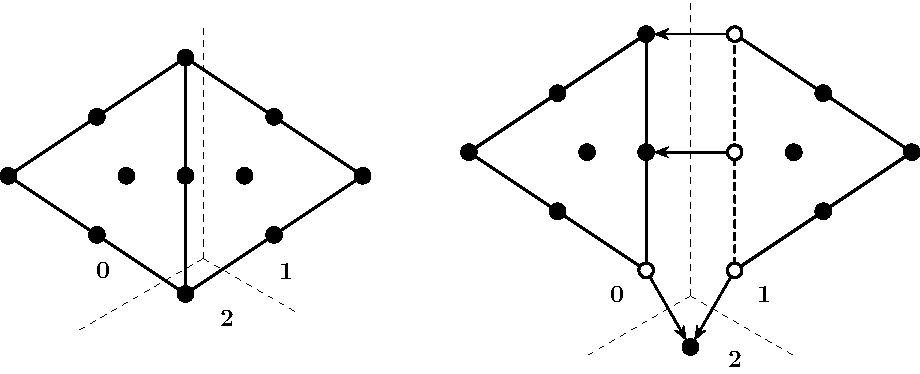
\includegraphics{star_forest_point.pdf}
  \caption{
    Global (left) and process-local (right) views of a mesh partitioned between three processes.
    The black dots represent the different mesh entities (the \emph{points}).
    Ghost points are shown as hollow circles.
  }
  \label{fig:dmplex_split_mesh}
\end{figure}

DMPlex works in distributed memory environments by partitioning the entire global mesh into local pieces that are kept on each process.
To enable stencil calculations \emph{ghost} points are duplicated across processes.
An example partitioned mesh is shown in \cref{fig:dmplex_split_mesh}.

\begin{figure}
  \centering
  \begin{subfigure}[t]{.45\textwidth}
    \centering
    \includegraphics{star_forest_abstract_mesh.pdf}
    \caption{Star forest suitable for describing the point ownership in \cref{fig:dmplex_split_mesh}.}
    \label{fig:star_forest_abstract_mesh}
  \end{subfigure}
  \hspace{1em}
  \begin{subfigure}[t]{.45\textwidth}
    \centering
    \includegraphics{star_forest_abstract_global.pdf}
    \caption{Star forest encoding the communication pattern of a globally consistent value shared between 7 processes.}
    \label{fig:star_forest_abstract_global}
  \end{subfigure}
  \caption{
    Common star forest patterns.
    Each point is labelled with its owning process and root and leaf points are shown in black and white respectively.
  }
\end{figure}

Parallel communication in DMPlex is handled by \emph{star forests}~\cite{zhangPetscSFScalableCommunication2021}.
Star forests relate equivalent points across processes as a collection (forest) of depth-1 trees (stars) consisting of a single \emph{root} and any number of \emph{leaves}.
They support two main operations: \emph{broadcasts} from roots to leaves and \emph{reductions} from leaves to roots.

Star forests are a powerful abstraction for describing a range of different parallel communication patterns.
For example,  a value shared globally across $n$ processes can be represented as a star forest containing a single star, with the root node on process 0 and $n-1$ leaves, 1 for each other process (\cref{fig:star_forest_abstract_global}).
For distributed meshes, star forests encode point ownership by making each shared point into a separate star, with the owning process the root and ghost processes the leaves.
A sketch of the star forest encoding the point ownership for the partitioned mesh in \cref{fig:dmplex_split_mesh} is shown in \cref{fig:star_forest_abstract_mesh}.
DMPlex refers to this object as the \emph{point star forest}.

\begin{figure}
  \centering
  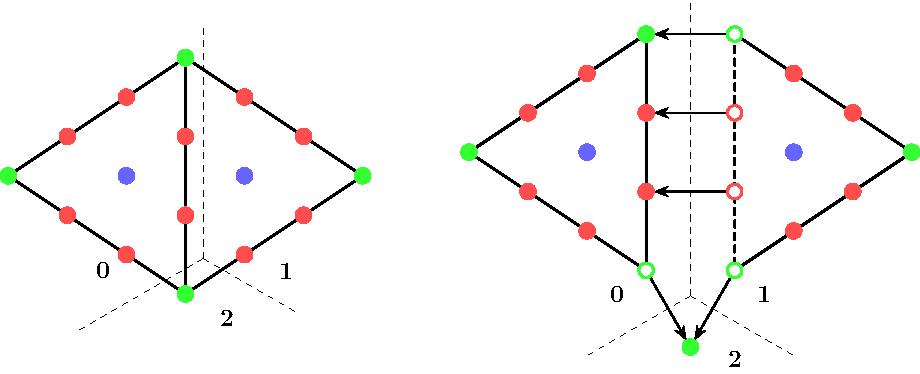
\includegraphics{star_forest_dof.pdf}

  \caption{
    Global (left) and process-local (right) views of a $P_3$ function space partitioned between three processes.
    Ghost DoFs are shown as hollow circles.
  }
  \label{fig:dmplex_split_function_space}
\end{figure}

To share parallel data, instead of points, the point star forest is not suitable because the number of DoFs per point is variable.
A new star forest, called the \emph{DoF star forest}, is therefore created.
To produce it, DMPlex composes the point star forest with the \ccode{PetscSection} encoding the data layout.
\Cref{fig:dmplex_split_function_space} shows an example of how mesh data might be shared between processes.

\section{\pyop2}

% NOTE: should mention extruded (then mention at end of doc)

As first introduced in \cref{sec:intro_existing_software}, \pyop2 is a library for doing mesh stencil calculations~\cite{rathgeberPyOP2HighLevelFramework2012}.
It was originally introduced to provide the same abstractions as OP2~\cite{mudaligeOP2ActiveLibrary2012}, but use runtime code generation instead of source-to-source translation.
It is a core component of the Firedrake finite element framework~\cite{FiredrakeUserManual}.

\subsection{Data structures}

\begin{table}
  \centering
  \begin{tblr}{|[1pt]l|[1pt]l|[1pt]l|[1pt]l|[1pt]}
    \hline[1pt]
    & \pycode{Global} & \pycode{Dat} & \pycode{Mat} \\
    \hline[1pt]
    Usage & Globally constant value & Distributed vector & Distributed matrix \\
    \hline[1pt]
    Constructor & \pycode{GlobalDataSet} & \pycode{DataSet} & 2 \pycode{DataSets} \\
    \hline[1pt]
    Storage type & \numpy{} array & \numpy{} array & PETSc \ccode{Mat} \\
    \hline[1pt]
  \end{tblr}
  \caption{\pyop2 global data structures.}
  \label{tab:pyop2_data_types}
\end{table}

Summarised in \cref{tab:pyop2_data_types}, \pyop2 has three supported data structures: \pycode{Globals} (constants), \pycode{Dats} (vectors), and \pycode{Mats} (matrices).
Like \numpy{}, each of these are implemented by coupling `simple' data structure to metadata that provides additional semantic information.
In \pyop2 this metadata is called a \emph{data set}.
Internally, \pycode{Globals} and \pycode{Dats} both use \numpy{} arrays to store data, whereas \pycode{Mats} use PETSc matrices (that are also called \ccode{Mats}).

For multi-field problems such as the Stokes example in \cref{chapter:background} \pyop2 has \emph{mixed data sets}, which are simply a collection of regular data sets.
Mixed data sets produce \pycode{MixedDats} which are, again, simply a collection of regular \pycode{Dats}.
An example of a \pyop2 data layout for a multi-field problem is shown in \cref{fig:scott_vogelius_element_dof_layout_pyop2}.
Observe that, since the DoFs are associated with multiple mesh entities, data are stored on a \emph{node set}, losing topological information.

\subsection{Parallel loops}
\label{sec:pyop2_parallel}

\begin{listing}
  \centering
  \caption{Code to construct and execute a \pyop2 parallel loop.}
  \begin{minipage}{.9\textwidth}
    \begin{pyalg2}
      par_loop(kernel,                          # local kernel
               src_set,                         # iteration set
               dat0(READ, src_to_target_map),   # arguments
               dat1(WRITE, src_to_target_map))  #    "
    \end{pyalg2}
  \end{minipage}
  \label{listing:pyop2_parloop_demo}
\end{listing}

In order to apply kernels to these data structures, a \emph{parallel loop} is constructed and executed.
The loop takes as arguments a \emph{local kernel}, \emph{iteration set} and any number of \emph{arguments} that specify the pack/unpack instructions needed to prepare data for the local kernel.
Constructing a parallel loop requires an invocation like that shown in \cref{listing:pyop2_parloop_demo}.
\pycode{kernel} is the local kernel representing the stencil operation to be performed per iteration, \pycode{src_set} is the set that is iterated over (termed the \emph{iteration set}), and \pycode{dat0} and \pycode{dat1} are \pycode{Dat} objects that are passed through to the local kernel.
\pycode{kernel} may be either a string of C code or a \emph{loopy kernel} (see \cref{sec:pyop2_codegen}).
Both \pycode{Dats} associate data with some \pycode{target_set} and hence are addressed with a map relating these sets (\pycode{src_to_target_map}).
\pycode{dat0} is accessed using the \pycode{READ} access descriptor, meaning that it only needs to be packed and passed into the local kernel, whereas \pycode{dat1} is accessed with \pycode{WRITE}, so it only requires unpacking.

\subsubsection{Interleaving computation and communication}
\label{sec:pyop2_interleave}

\begin{algorithm}
  \caption{The \pyop2 parallel loop execution algorithm to interleave computation and communication.}
  %
  \begin{algorithmic}[1]
    \State \Call{BeginHaloExchanges}{} \Comment{Begin sending halo data}

    \For{\textit{item} \textbf{in} \textit{iterset.core}} \Comment{Do the computations that \textbf{do not} need halo data}
      \State \Call{Compute}{\textit{item}}
    \EndFor

    \State \Call{AwaitHaloExchanges}{} \Comment{Wait for halo exchanges to complete}

    \For{\textit{item} \textbf{in} \textit{iterset.owned}} \Comment{Do the computations that \textbf{do} need halo data}
      \State \Call{Compute}{\textit{item}}
    \EndFor
  \end{algorithmic}
  \label{alg:pyop2_comp_comm_overlap}
\end{algorithm}

By keeping careful track of the parallel decomposition of sets, \pyop2 is capable of interleaving computation and communication when executing parallel loops.
To do so each set is split, by the user, into 3 parts:
\begin{description}
  \item[\coreiter{}]
    Set elements that do not require any data from other processes during a parallel loop.
  \item[\ownediter{}]
    Set elements that are owned by the current process but require data from other processes.
  \item[\ghostiter{}]
    Set elements present on a process that belong to another process.
\end{description}
From this partitioning it is possible to interleave computation and communication.
Computations over \coreiter{} points do not read any ghost data, and hence can be executed without waiting for any communication to complete, whereas \ownediter{} points need valid ghost data and so must wait for all communication to be completed before beginning.
This is shown in \cref{alg:pyop2_comp_comm_overlap}.
\ghostiter{} points are not iterated over.

To facilitate this algorithm, \pyop2 arranges sets, and thus stores data, in a partitioned manner, where \coreiter{} points precede all \ownediter{} points and all \ownediter{} precede all \ghostiter{} points:
\begin{center}
  \includegraphics{pyop2_partition.pdf}
\end{center}

\subsubsection{Limitations}
\label{sec:pyop2_parallel_limitation}

Arranging the data like this is problematic for one key reason: it conflates the partitioning of the data layout (\ghostiter{}/non-\ghostiter{}) with that of the iteration set (\coreiter{}/\ownediter{}).

The partitioning of \ghostiter{}/non-\ghostiter{} points comes from the star forest description of the parallel overlap, and hence is known \emph{when the array is initialised}.
It therefore makes sense to embed this information in the data layout.
By contrast, \ownediter{} points are defined as being points that need ghost data in order to be executable.
\emph{This is dependent upon the stencil}.
Differently sized stencils touch different numbers of adjacent points, changing the \coreiter{}/\ownediter{} partitioning.
\pyop2 will therefore not work correctly in parallel for programs that use several different stencil sizes acting on the same data.

\begin{figure}
  \centering
  \includegraphics[scale=2]{pyop2_issue.pdf}
  \caption{
    Example illustrating the issues that occur when assigning \coreiter{}/\ownediter{} labels based solely upon the iteration set.
    In this example one loops over the cells of a partitioned quadrilateral mesh (black) and accesses data defined on a mesh of disconnected vertices (blue), which has a different parallel distribution.
    Ghost edges and vertices are marked with dashes and hollow circles respectively.
    Cells with the label \coreiter{} are marked with a \textbf{C} and those with \ownediter{} are marked with a \textbf{O}.
    The problematic cells, which would be erroneously labelled as \coreiter{} instead of \ownediter{}, are marked with a \textbf{?}.
  }
  \label{fig:pyop2_issue}
\end{figure}

Further, the partitioning of \coreiter{}/\ownediter{} points is associated with the \emph{iteration set}, instead of the data structures.
This means that \pyop2 cannot do the right thing for cases where data structures do not share the same parallel decomposition (e.g. when transferring data between meshes).
Stencils may touch only non-\ghostiter{} points on one mesh, leading to the iterate being classified as \coreiter{}, but they may be \ghostiter{} on the other mesh, and hence the iterate ought to be labelled \ownediter{}.

This issue is demonstrated in \cref{fig:pyop2_issue}.
Given two meshes, one a quadrilateral mesh (black) and the other a mesh of disconnected vertices (blue), with differing parallel distributions, and assuming a loop over cells, it can be seen that it is possible for the \coreiter{}/\ownediter{} labels to be erroneously applied.
Specifically, the cells marked with \textbf{?} would be considered \coreiter{} by \pyop2 despite needing to access ghost DoFs from the vertex-only mesh.

\subsection{Code generation}
\label{sec:pyop2_codegen}

\begin{figure}
  \includegraphics[width=\textwidth]{pyop2_codegen_flowchart.pdf}
  \caption{Simplified code generation pathway for a \pyop2 parallel loop.}
  \label{fig:pyop2_codegen}
\end{figure}

To turn abstract parallel loop definitions into executable, fast code, \pyop2 utilises run-time code generation.
First, the parallel loop is \emph{lowered} to loopy, which is then lowered to C code and compiled to a binary.
This binary may then be called passing in the arguments from the original parallel loop.
This process is summarised in \cref{fig:pyop2_codegen}.

\subsubsection{Loopy}

Loopy~\cite{klocknerLooPyTransformationbased2014}, a polyhedral-model-inspired code generation library written in Python, is the primary intermediate representation of \pyop2.
Given a parallel loop, \pyop2 generates a loopy \pycode{LoopKernel} which is then lowered to C code and compiled.

In order to construct a \pycode{LoopKernel} the user needs to provide \emph{domains} (loops), \emph{instructions}, and \emph{arguments} (data passed into the kernel).
For the parallel loop in \cref{listing:pyop2_parloop_demo}, the \pycode{LoopKernel} and generated C code are shown in \cref{listing:pyop2_example_loopy_kernel} and \cref{listing:pyop2_example_c_code} respectively.
The local kernel, here omitted, is also (usually) a \pycode{LoopKernel} and would be included in the generated code as a separate function.

Given its high level of abstraction, loopy is a convenient target for \pyop2 for a number of reasons:
\begin{itemize}
  \item
    \pycode{LoopKernels} may be transformed to apply optimisations such as loop tiling, common subexpression elimination and vectorisation~\cite{klocknerLooPyFortran2015,klocknerArrayProgramTransformation2016,sunStudyVectorizationMatrixfree2020}.
  \item
    Code may be generated for targets other than CPUs including the GPU languages OpenCL~\cite{stoneOpenCLParallelProgramming2010a} and CUDA~\cite{CUDAProgrammingGuide}.
    This means that \pyop2 is capable of executing parallel loops on GPUs without making intrusive changes to the code - a fact demonstrated (as a proof-of-concept) by \cite{fenics2021-kulkarni}.
\end{itemize}

\begin{listing}
  \centering
  \begin{minipage}{.9\textwidth}
    \inputminted[linenos]{text}{./scripts/artefacts/pyop2_example_loopy_kernel_tidy.txt}
  \end{minipage}
  \caption{
    Abbreviated textual representation of the loopy kernel generated for the example parallel loop in \cref{listing:pyop2_parloop_demo}.
    The pack and unpack instructions are shown on lines 29 and 33 respectively.
  }
  \label{listing:pyop2_example_loopy_kernel}
\end{listing}

\begin{listing}
  \centering
  \begin{minipage}{.9\textwidth}
    \inputminted[linenos]{c}{./scripts/artefacts/pyop2_example_c_code_tidy.c}
  \end{minipage}
  \caption{
    The C code generated from the loopy kernel in \cref{listing:pyop2_example_loopy_kernel}.
    The pack and unpack instructions are shown on lines 13 and 20 respectively.
  }
  \label{listing:pyop2_example_c_code}
\end{listing}

\subsection{Limitations}

As an abstraction for mesh stencil computations, \pyop2 is limited because of its inflexible interface.
Not all mesh operations are expressible as a single kernel executed within a single loop.
For instance, algorithms for physics-based preconditioners such as hybridisation~\cite{gibsonSlateExtendingFiredrake2020} and additive Schwartz methods~\cite{farrellPCPATCHSoftwareTopological2021} involve multiple kernels and nested loops.
Though each has been implemented with \pyop2 and Firedrake, sui-generis code has been needed making the resulting software harder to compose.

One of the main reasons for this limiting interface is the fact that set-based approaches for describing mesh data \emph{discard important topological information}.
This makes it harder to build a composable interface because it creates a divide between the natural language for expressing mesh stencil algorithms - the mesh entities - and the description of how data are stored - on the nodes.

\section{Outlook}

In this chapter we introduced three existing pieces of software: \pyop2, \numpy{}, and PETSc DMPlex.
\pyop2 is a powerful library for automating mesh stencil calculations but weaknesses in its ability to describe mesh data limit its expressivity and hence certain mesh stencil algorithms cannot be described.
\numpy{} and DMPlex both provide abstractions for describing different types of data: \numpy{} describing fully structured, hierarchical N-dimensional arrays and DMPlex describing fully unstructured mesh data.

In this thesis we seek a unifying abstraction for mesh data, combining elements of \numpy{} and DMPlex, which may then be implemented in a mesh stencil package reusing concepts from \pyop2.
The new abstractions, called \emph{axis trees} and \emph{index trees} are discussed in \cref{chapter:axis_trees,chapter:indexing}, and the new mesh stencil package, called \pyop3, is introduced in \cref{chapter:pyop3}.

\end{document}
